% Analytic illustration only. c = 299792458 m/s.
% B in GHz, nominal monostatic resolution in cm = 14.9896229/B.
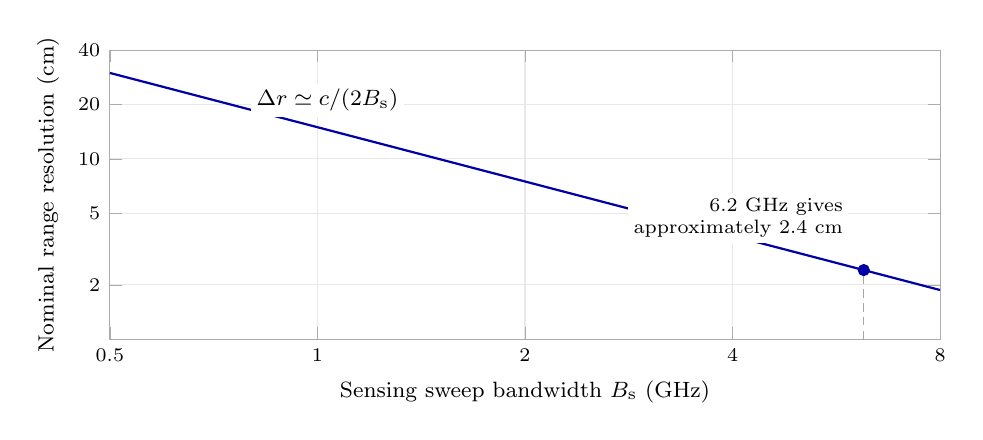
\begin{tikzpicture}
\begin{axis}[
  width=\columnwidth,height=5.25cm,
  xmin=0.5,xmax=8,ymin=1,ymax=40,
  xmode=log,ymode=log,
  xlabel={Sensing sweep bandwidth $B_{\mathrm{s}}$ (GHz)},
  ylabel={Nominal range resolution (cm)},
  xtick={0.5,1,2,4,8},xticklabels={0.5,1,2,4,8},
  ytick={2,5,10,20,40},yticklabels={2,5,10,20,40},
  tick label style={font=\scriptsize},
  label style={font=\footnotesize},
  grid=major,grid style={gray!18},
  axis line style={gray!65},tick style={gray!65},
  minor tick num=0,clip=false]
\addplot[blue!65!black,thick,domain=0.5:8,samples=100] {14.9896229/x};
\addplot[only marks,mark=*,mark size=2pt,blue!65!black]
  coordinates {(6.2,2.417681113)};
\draw[densely dashed,gray!70] (axis cs:6.2,1) -- (axis cs:6.2,2.417681113);
\node[anchor=south west,font=\footnotesize,fill=white,inner sep=2pt]
  at (axis cs:0.8,17) {$\Delta r \simeq c/(2B_{\mathrm{s}})$};
\node[anchor=south east,font=\scriptsize,align=right,fill=white,inner sep=2pt]
  at (axis cs:5.9,3.4) {6.2 GHz gives\\approximately 2.4 cm};
\end{axis}
\end{tikzpicture}
